\chapter{System test results}
The signal conditioning system was implemented successfully as can be seen in Figure \ref{fig:system_picture}, all of the sub circuits were tested under various circumstances and passed all of the design requirements with minimal noise interferance. A system test summary can be seen in Table \ref{tab:powersupplytable} showing the total current supplied by the respective power supplies to the signal conditioning circuitry, as well as the voltage level of these power supplies.

\begin{figure}
    \centering
    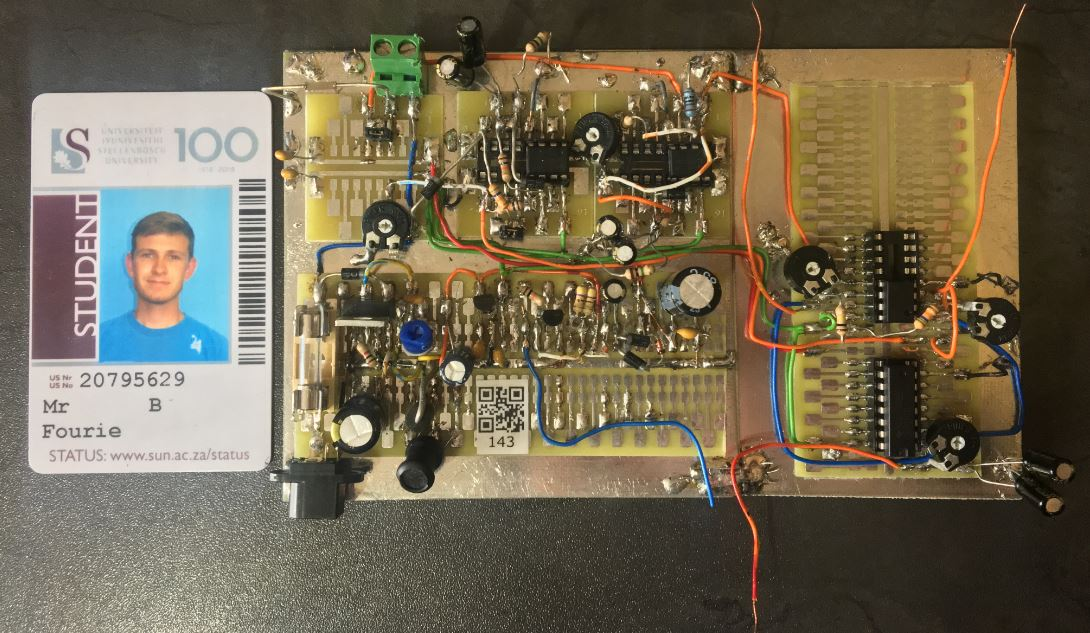
\includegraphics[width = 0.6\linewidth]{Figures/system_picture.JPG}
    \caption{Signal Conditioning Circuitry}
    \label{fig:system_picture}
\end{figure}

\begin{table}
        \centering
        \footnotesize
        \caption{Table showing system test summary.}
         \begin{tabular}{|C{2.5cm}|C{2cm}|C{2.7cm}|C{2.7cm}|}
          \hline
           Regulator & Rail Voltage ($\SI{}{V_{peak}}$) &  Current Supplied ($\SI{}{mA_{peak}}$) & Measured Noise ($\SI{}{mV_{peak}}$) \\
           \hline
           $\SI{5}{V}$ regulator    & 5.04    & 22.09    & 4.71   \\
           $\SI{-5}{V}$ regulator   & -5.12   &  0  & 3.53  \\
          \hline
        \end{tabular}
     \label{tab:powersupplytable}
\end{table}












